\TOWRITE{ALL}{Proofread 3.3 pass 2}
\label{sect:mgt}

The management and decision-making approach of \TheProject has been
tailored to the real needs of the project and \emph{overcomplexity has been avoided
in favour of an efficient management organisation able to effectively guarantee
project success}. To this end, the number of committees has been kept to
the minimum and the rules will be flexible whilst still providing a good basis
for efficient implementation of the project.

Project management activities in \TheProject comprise a wide array
of activities, including scientific and administrative management,
guidance on decision making, contractual management, financial
management, supervision of and compliance with ethical standards,
management of knowledge and IPR issues, and coordination of
communication activities. Most partners have extensive experience
with EU funded projects, while two SMEs are recent start-ups.
\TheProject management will thus be tailored to varying needs and
requirements of individual partners.

\subsubsection{Management}

The project will be coordinated by \site{SRL},
represented by Benjamin Ragan-Kelley (Project Coordinator),
who has been a developer and leader in the Jupyter project since its inception in 2014,
and IPython before that,
and a site and work package leader in prior H2020 project, OpenDreamKit,
and currently leads the JupyterHub and Binder open source projects
in the Jupyter community.

The Project Coordinator will be assisted by a part-time (50\%) Project
Manager, Katarina Subakova, who has significant experience with Horizon 2020, both
as a project manager and as a head of Horizon 2020 Helpdesk.
Additional feedback and expertise will be brought by Financial, Legal
and European affairs officers from Simula.

In addition, Hans Fangohr will act as Project Deputy, being constantly
updated by the coordinator and manager on the project evolution in
order to be able to temporarily take over the coordination in case the
coordinator would be incapacitated.

\subsubsection{Organisational structure and decision-making}

\begin{figure}
  \centering
  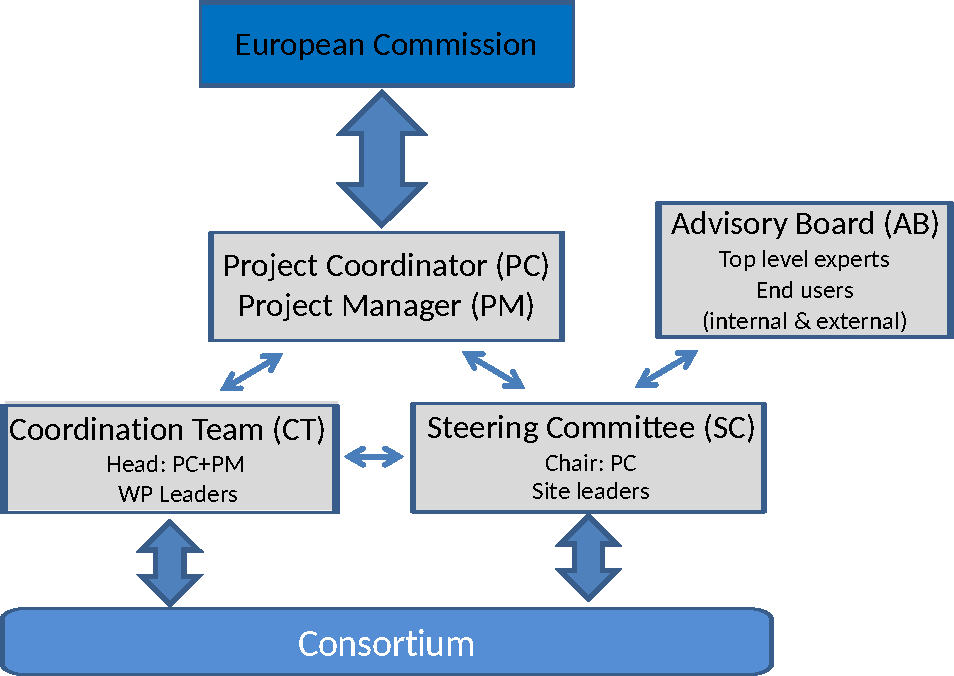
\includegraphics[width=0.75\textwidth]{management_structure.pdf}
  \caption{Management structure}
  \label{figure.management}
\end{figure}

The organisational structure, shown in the Figure~\ref{figure.management}, has been designed
to enable efficient coordination of the project --- the
development and evaluation of an Open Science toolkit
integrating several previously separated tools and software and
involving both academic actors and industrial stakeholders. It is jointly agreed on
by \TheProject consortium and adapted to its size and composition,
the tasks and duties of all partners involved.

We have designed the management structure and procedures to deal in a
flexible manner with the following challenges:
\begin{compactitem}
\item to integrate all consortium members and to mobilise their
  expertise, knowledge and networks at every stage of the project;
\item to give the maximum attention to the end-users needs and
  requirements;
\item to continuously involve expertise and knowledge of relevant
  stakeholders and their networks, and
\item to efficiently coordinate the project implementation in a
  collaborative environment and ensure its sustainability.
\end{compactitem}

The design has been largely adapted from that of OpenDreamKit which
has proved very effective for this type of project, with some
simplification as suggested by past experience:
\begin{itemize}
\item Suppression of the Quality Review Board: its role can
  effectively be subsumed by the steering committee; also the head of
  OpenDreamKit's Quality Review Board, Hans Fangohr, will carry over
  the accumulated experience and best practices, and the lessons
  learned from the OpenDreamKit quality review board will be shared
  within the BOSSEE consortium.
\item Suppression of the End User Group: as in OpenDreamKit, all
  participants are either end users themselves, or in close contact
  with such end users. To guarantee the effectiveness of this
  simplified structure, we include end users in the advisory board.
\end{itemize}


The coordinator acts as an intermediary between the Partners and
the European Commission. The coordinator will oversee the project
planning, monitor that execution is carried out in time and that
the objectives are achieved and closely interact with the project
officer for project monitoring and delivery of the performance
indicators.  The Project Manager will ensure  efficient day-to-day
management of the project, reporting, feedback to partners on
administrative, financial and legal issues, tracking of  resource
allocation and consumption, and communication inside and outside the
consortium.

The resources of all partners will be mobilised by decentralisation of
responsibilities through the assignment of leadership for work
packages. Clear distribution of tasks, efficient decision making
mechanisms and a sound financial management will safeguard the
achievement of the project's objectives.

\ifgrantagreement\else
\subsubsection{Milestones}
For a description of the milestones and their motivations see
Section~\ref{sec:milestones}; a tabulation of the milestones, which work packages
are involved, and a means of verification can be seen in Table~\ref{tab:milestonetable}.

\milestonetable
\fi

\subsubsection{Project roles}

%Project Coordinator and Project Manager can meet any time and at least
%twice a week.

The following bodies will form the organisational structure of the
\TheProject project : Coordination Team (CT), Steering Committee (SC),
Advisory Board (AB).%, End User Group (EUG) and Quality Review board (QRB).

\begin{description}
\item{\textbf{Coordination Team (CT)}} \nobreak\par
\textbf{Members:} The CT is composed of the Work Package leaders
and headed by the Project Coordinator, assisted by the Project
Manager.

\textbf{Responsibilities:} The CT is an executive body in charge of
the project implementation and monitoring.
It takes operational decisions necessary for the smooth execution of
the project.

\textbf{Tasks:}
\begin{compactenum}
\item Monitoring the timely execution of the tasks and achievement of
  the objectives;
\item Preparation of scientific and financial progress reports;
\item Controlling Work Package progress by assessing it through technical
  reports developed by the partners;
\item Making proposals to the Steering Committee of re-allocation of
  tasks, resources and financial needs for the fulfilment of the work
  plan;
\item Preparing the drafts and validating the project deliverables to
  be submitted to the Commission.
\end{compactenum}

\textbf{Meetings:} The coordination team will meet every 6 months.
If necessary, extra meetings will be arranged.

\item{\textbf{Steering Committee (SC)}}\nobreak\par

\textbf{Members:} The SC is chaired by the Project Coordinator
and includes one representative from each partner organisation.

\textbf{Responsibilities:} The SC is the decision-making body in
charge of the strategic orientation of the project.  It takes decisions on scientific
directions, re-allocation of resources, consortium
changes and intellectual property rights.

\textbf{Meetings:} Annual meetings. If necessary, extra-meetings
will be arranged.  Written minutes of each meeting will be produced,
which shall be the formal record of all decisions taken. A procedure
for comment and acceptance is proposed.

\textbf{Voting procedure:} The SC shall not deliberate until a quorum
of three-fourth (3/4) of all Members are present (possibly through
video-conference) or represented. Each Member shall have one vote. The
SC will work on consensual decisions as much as possible and resort to
voting only if unavoidable. Voting decisions shall be taken by a
majority of two-thirds (2/3) of votes with quorum two-thids (2/3) of
the whole set of members. Exceptional decisions (large changes to the
budget ($\geq$ 100k euros), evolution to the consortium, firing the
coordinator, resolving ambiguity about whether something is a hard
question) shall be taken by a majority of three-fourth (3/4) of votes
with quorum three-fourth (3/4) of the whole set of members. Votes can
be electronic.

\item{\textbf{Advisory board (AB)}} \nobreak\par

  \textbf{Members:} top level experts and end-users from partner and
  external organisations, from a variety of disciplines and both from
  academic and industrial sector. Together, they have a deep
  understanding of both market and technical problems, and an
  awareness of opportunities

  \textbf{Responsibilities:} to give an independent opinion on
  steering, scientific and innovation matters, in order to guaranty
  quality implementation of the project, adequateness to the end-users
  needs, efficient innovation management, and project sustainability.

  % \textbf{Tasks:} to control the project execution from the point of
  % view of the end user needs and requirements, to test the tool and to
  % detect its potential shortcomings at the early stages, to propose
  % adaptation measures.

  \textbf{Meetings:} at the request of the Steering Committee, including attending annual project meetings.
\end{description}

\subsubsection{Project management tools and procedures}

Project partners and management bodies will communicate through
a dedicated project web platform, maintained by the Project
Manager. WP leaders will monitor progress of
participants of their WP at least monthly, and participants will inform their WP
leaders when problems are encountered. Major problems will be
discussed in (teleconference) meetings with the Project Coordinator
and Project Manager. Each WP leader will be free to organise
extra meetings with WP partners, if necessary. Scientific and
financial progress reports will be collected, assembled and
transmitted to the Project Coordinator by the WP leaders through the
web platform. On basis of the Progress Reports, the Coordination Team
will monitor progress of the project, identify bottlenecks and find
solutions for these problems. Where needed, adaptations to the project
plan will be made, with the aim of ensuring the delivery of the project
results as agreed with the EC. Major adaptations need to be approved
by the Steering Committee.

The Coordination Team, will ensure efficient innovation management.
They will carefully monitor new opportunities in order to suggest, if
necessary, to new directions to the Steering Committee. For legal
aspects, the latter will have a feedback from legal officers from the
Coordinator’s European affairs office,
specialised in Intellectual Property.

Our management structure and procedures will ensure that our network
of partners from both academic and industrial sectors is focused at
achieving the promised tasks and deliverables, efficiently managing
the innovation process and largely opening the developed tools,
insights and services to the EOSC and its final users.
The partners will sign a Consortium Agreement, in which operational
rules and decision making procedures will be laid down.

\emph{CONFLICT RESOLUTION} - For the cases where contentious decisions
need to be made, or conflicts are arising which cannot be solved bilaterally,
steps to prevent further escalation and procedures to resolve disputes
and decision-making procedures are laid down in the Consortium Agreement.
In case of conflicts or a needed decision in a task or work package,
the WP Leader shall resolve the conflict and agree on a solution or decision.
If a solution of the conflict cannot be found or if a Party does not accept
the proposed solution, the issue must be forwarded to the Steering committee (SC),
which in its turn will try to resolve the issue together with the conflicting parties
within 10 working days. If no agreement can be reached, the Project Coordinator (PC) can
base its decision on the 2/3 majority vote of the SC or take a different decision.
In any case, the Coordinator will take the final decision. All parties will make
efforts that decisions are resolved at a level as low as possible.

\subsubsection{Quality and Innovation management}

\TheProject Project Quality Management will ensure that
the project meets a high quality level as well as satisfying the EU commission
requirements. The basic approach to quality management is compatible with the
International Project Management standards and guidelines (PMI).

\begin{itemize}
\item Quality planning: internal standards from participants and national and international standards and
regulatory requirements will be considered to create the quality metric.
\item Quality control: the overall project performance will be evaluated on a regular basis to provide
confidence that the project satisfies the expectation and EU provisions.
\item Quality assurance: specific project results will be monitored to determine if they comply with
expectations and eliminate causes of unsatisfactory performance. To this aim, deliverables have been
planned to give the necessary information and evidence that quality standards have been achieved.
\end{itemize}

In the context of the Responsible Research Innovation paradigm promoted by the European Commission in
the H2020 framework, \TheProject is willing to respond to societal desirability and societal acceptability
question identifying new opportunities in the Open Science hub through innovation that is in the public
interest. \TheProject consortium recognises innovation as an essential element for driving business growth
and maintaining competitive advantage. The innovation management work will prevent that \TheProject
results suffer from missing expected functionalities, which would lead to user dissatisfaction, and will
ensure that the ethical and societal aspects are incorporated into the design process from the beginning.

\subsubsection{Risks and risk management strategy}\label{sec:risks}

The risk in the project execution as planned is carefully assessed and
managed. We base our plans on long standing experience, and we bring
together the world's experts in the relevant tools and techniques.

A key feature of this project is the involvement of a wide set of
partners from multiple domains. While this ensures complementary
coverage of a wide set of skills and provides robustness in different
ways, we will have to ensure that all partners work as closely knit
team. 

Our open source approach means that all our code and outputs
are open and visible to anybody at sites like GitHub and bitbucket
throughout the project. In particular, it is common for users and external collaborators of
computational and infrastructure software to use the leading edge versions, thus
beta-testing code in-between major releases to identify bugs and potential security risks
early on. This results in risk reduction: where our design decisions or technical approaches are
controversial, this will be detected early by those users, giving the
consortium useful feedback to consider.

As part of the Management Work Package, and with support from the
Coordination Team, the project coordinator will maintain and regularly
update a Risk Management Plan; at the end of each Reporting Period,
this updated plan will be included in the project's Technical Report.

It will identify and categorise all
potential strategic risks (legal, financial, human resources risks, etc)
to the successful delivery of the project, their probability and impact.
For each risk area, mechanisms for risk mitigation will be identified
and contingency actions will be proposed.

Risks will be evaluated in terms of project goals and objectives,
according to the following four steps:
\begin{enumerate}
\item Identification of risks using a structured and rational approach to
ensure that all areas are addressed.
\item Quantitative assessment and ranking of the risks.
\item Definition of procedure to reduce (or minimize) risk.
\item Monitoring and management of risks throughout the project life
with milestone review and reassessment.
\end{enumerate}

Finally, as reported above, a conflict resolution mechanism will be put in place.
Whereby decision making divergence and conflicts that cannot be solved at the
SC level will be submitted to the Coordinator. The
mediation and resolution process used is the following:
\begin{itemize}
\item Case presented by the involved parties.
\item Development of a fact-based and neutral report by the coordinator
to be provided to the conflicting parties and SC.
\item Final decision to resolve the conflict made by SC.
\end{itemize}

\ifgrantagreement\else
An initial risk assessment appears as Figure~\ref{risk-table}.

\TOWRITE{ALL}{risk about EOSC integration}

\begin{figure}
\begin{center}
\begin{tabular}{|m{.2\textwidth}|m{.12\textwidth}|m{.58\textwidth}|}\hline
  Risk & Level with / without mitigation & Mitigation measures
  \\\hline

   \multicolumn{3}{|c|}{
    \textit{General technical / scientific risks}
   }
   \\\hline

  Implementing infrastructure that does not match the needs of end users & High/Low &
  Many of the members of the consortium are themselves end-users with
  a diverse range of needs and points of views; hence the design of
  the proposal and the governance of the project is naturally steered
  by demand; besides, because we provide a toolkit, users have the
  flexibility to adapt the infrastructure to their needs. In addition, the open source nature 
  of the project facilitates and promotes the involvement of the wider community in terms of 
  providing feedback and requesting additional features via platforms such as GitHuib and BitBucket 
  on a regular basis. 
  \\\hline

  Lack of predictability for tasks that are pursued jointly with
  the community & Medium/Low &
  The PI's have a strong experience managing community-developed
  projects where the execution of tasks depends on the availability of
  partners. Some tasks may end up requiring more manpower from
  \TheProject to be completed on time, while others may be entirely
  taken care of by the community. Reallocating tasks and redefining
  work plans is common practice needed to cater for a
  fast evolving context. Such random factors will be averaged out over
  the large number of independent tasks.\\\hline

  Reliance on external software components & Medium/Low & The non trivial
  software components \TheProject relies on are open source. Most are
  very mature
  and supported by an active community, which offers strong long run
  guarantees. The other components could be replaced by alternatives, or
  worst comes to worst, taken over by the participants.
  \\\hline

%  \multicolumn{3}{|c|}{
%    \textit{Use-case risks}
%  }
%  \\\hline
%
%  & & \TOWRITE{WP4}{Risks related to use-cases in WP4}
%  \\\hline

  \multicolumn{3}{|c|}{
    \textit{Management risks}
  }
  \\\hline

  Recruitment of highly qualified staff & High/Medium &

  Great care was taken coordinating with currently running projects to
  rehire personnel with strong track record, and identifying pool of
  candidates to hire from, notably in the developers community of
  software related to the project. This was favored by the partners'
  long history of training and outreach activities. In addition, we
  have a critical mass of qualified staff in the project enabling us
  to train and mentor new recruits.

 \\\hline

  Different groups not forming effective team & Medium/Low & Long
  track record of working collaboratively on code across multiple
  sites. Aggressive planning of project meetings, workshops and
  one-to-one partner visits to facilitate most effective teamwork,
  combining face-to-face time at one site with remote
  collaboration.\\\hline
  % this also justifies our generous travel budget.

  Partner leaves the consortium & Low/High & If the GA requires a replacement
  in order to achieve the project's objectives, the consortium will invite a new
  relevant partner in. If a replacement is not necessary, the resources and tasks
  of the departing partner will be reallocated to the alternative ones within the
  consortium.
  \\\hline

  \multicolumn{3}{|c|}{
    \textit{Dissemination risks}
  }
  \\\hline

  Impact of dissemination activities is lower than planned. & Low/Medium &

  Partners in the consortium have a proven track record at community
  building, training, dissemination, social media communication, and
  outreach, which reduces the risk. The Project Coordinator
  will monitor impact of all dissemination activities. If a deficiency is identified, the consortium
  will propose relevant corrective actions.\\\hline

  \end{tabular}
\end{center}
\caption{\label{risk-table}Initial Risk Assessment}
\end{figure}
\fi
%\TOWRITE{NT/Eugenia}{Impredictability}

%\includegraphics[width=.94\textwidth]{Pictures/Impact-img1.png}

%   But: since Open Source softwares are freely accessible, security
%   and privacy issues are a concern. Anytime a resource is shared,
%   there is greater risk of unauthorised access and contaminated data.
%   Providers must demonstrate security solutions, which should include
%   physical security controlling access to the facility and protection
%   of user data from corruption and cyber attacks.}


\TOWRITE{ALL}{
  Add a paragraph about data management plan. What data will we produce, which data is available from the
  start, how do we handle it...
}

%  LocalWords:  mgt Paris-Sud UPSud Thiery Sage-Combinat decentralisation textwidth hline
%  LocalWords:  textwidth Jupyter slmhnlnhfnhs hsfhs ghshsh includegraphics unauthorised

%%% Local Variables:
%%% mode: latex
%%% TeX-master: "proposal"
%%% End:
%  LocalWords:  TOWRITE subsubsection organisational compactenum ipr Impredictability
%  LocalWords:  textbf nobreak smallbreak
